\ifdefined\COMPLETE
\else
\documentclass[12pt]{article}
\usepackage{tikz}
\usetikzlibrary{shapes, calc, arrows, through, intersections, decorations.pathreplacing, patterns}

\begin{document}
\fi

\def\alph{$2+\sqrt{5}$}
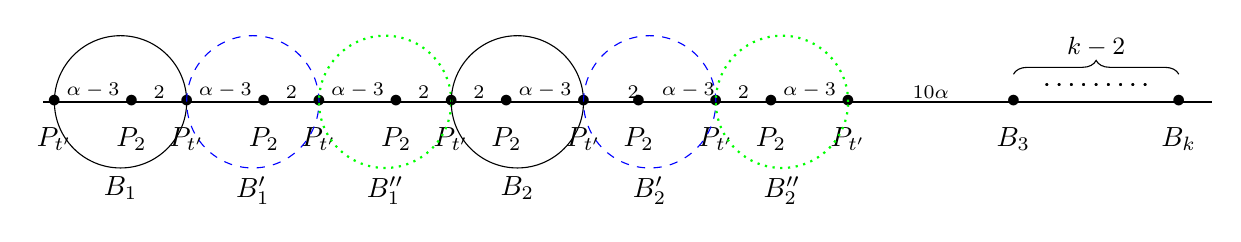
\begin{tikzpicture}[scale=7]
	\coordinate (x) at ($ (-0.02,{sqrt(0)}) $);
	\coordinate (y) at (2.1,0);
	\draw[thick] (x) --(y);

	\node[label=270:$P_{t'}$] at (0.0,0) {$\bullet$};
	\node[label={[yshift=-0.2cm]\scriptsize $\alpha-3$}] at (0.07,0) {};
	\node[label=below:{$P_2$}] at (0.14,0) {$\bullet$};
	\node[label={[yshift=-0.2cm]\scriptsize $2$}] at (0.19,0) {};
	\node[label=270:$P_{t'}$] at (0.24,0) {$\bullet$};
	\node[label={[yshift=-0.2cm]\scriptsize $\alpha-3$}] at (0.31,0) {};
	\node[label=270:$P_2$] at (0.38,0) {$\bullet$};
	\node[label={[yshift=-0.2cm]\scriptsize $2$}] at (0.43,0) {};
	\node[label=270:$P_{t'}$] at (0.48,0) {$\bullet$};
	\node[label={[yshift=-0.2cm]\scriptsize $\alpha-3$}] at (0.55,0) {};
	\node[label=270:$P_2$] at (0.62,0) {$\bullet$};
	\node[label={[yshift=-0.2cm]\scriptsize $2$}] at (0.67,0) {};
	\node[label=270:$P_{t'}$] at (0.72,0) {$\bullet$};	
	\node[label={[yshift=-0.2cm]\scriptsize $2$}] at (0.77,0) {};
	\node[label=270:$P_2$] at (0.82,0) {$\bullet$};	
	\node[label={[yshift=-0.2cm]\scriptsize $\alpha-3$}] at (0.89,0) {};
	\node[label=270:$P_{t'}$](B) at (0.96,0) {$\bullet$};	
	\node at (1.89,0.03) {$\ldots\ldots\ldots$};	
	\node[label=270:$P_2$] at (1.06,0) {$\bullet$};	
	\node[label=270:$P_{t'}$] at (1.2,0) {$\bullet$};	
	\node[label={[yshift=-0.2cm]\scriptsize $2$}] at (1.25,0) {};
	\node[label=270:$P_2$] at (1.3,0) {$\bullet$};	
	\node[label={[yshift=-0.2cm]\scriptsize $\alpha-3$}] at (1.37,0) {};
	\node[label=270:$P_{t'}$] at (1.44,0) {$\bullet$};	
	\node[label={[yshift=-0.2cm]\scriptsize $2$}] at (1.05,0) {};
	\node[label={[yshift=-0.2cm]\scriptsize $\alpha-3$}] at (1.15,0) {};
	\node[label={[yshift=-0.2cm]\scriptsize $10\alpha$}] at (1.59,0) {};
	\node[label=270:$B_3$](B) at (1.74,0) {$\bullet$};	
	\node at (1.89,0.03) {$\ldots\ldots\ldots$};	
	\node[label=270:$B_k$](p3end) at (2.04,0) {$\bullet$};	
	\node(A) at (1.89,0.1) {\small $k-2$};	
	
	\node[label=270:$B_1$] at (0.12,-0.1) {};	
	\node[label=270:$B_1'$] at (0.36,-0.1) {};	
	\node[label=270:$B_1''$] at (0.6,-0.1) {};	
	\node[label=270:$B_2$] at (0.84,-0.1) {};	
	\node[label=270:$B_2'$] at (1.08,-0.1) {};
	\node[label=270:$B_2''$] at (1.32,-0.1) {};	
	
	\draw (0.12,0) circle (0.12);
	\draw[dashed, blue] (0.36,0) circle (0.12);
	\draw[dotted, green, thick] (0.6,0) circle (0.12);
	\draw (0.84,0) circle (0.12);
	\draw[dashed, blue] (1.08,0) circle (0.12);
	\draw[green, thick, dotted] (1.32,0) circle (0.12);
	\draw[decorate,decoration={brace,amplitude=5pt}]
	(1.74, 0.05) -- (2.04, 0.05);
	%\draw (A) -- (1.74, 0.06);
\end{tikzpicture}


\ifdefined\COMPLETE
\else
\end{document}
\fi
